%========================================================================================
% Compilation should work with PDFLaTeX
%========================================================================================
% Type of document and general formatting
\documentclass[a4paper,11pt]{article}

\usepackage[left=2.5cm,right=2.5cm,top=2.5cm,bottom=2.5cm]{geometry}
\linespread{1.25}

%========================================================================================
% These packages are for language and font settings
\usepackage[english,activeacute]{babel} % Language
\usepackage{tgpagella}					% Text font
\usepackage[T1]{fontenc}				% T1 Encoding of font
\usepackage[utf8]{inputenc}				% Special symbols
\usepackage{lmodern}


%========================================================================================
\usepackage[sc]{mathpazo}				% Math font
\usepackage{amsmath,amsfonts,amssymb}	% Math symbols
\usepackage{dsfont}						% Math symbols like R for reals...
\usepackage{amsthm}						% For theorem styles
\usepackage{siunitx}

%========================================================================================
% Other packages
\usepackage{graphicx}
\usepackage{longtable}
\usepackage[svgnames]{xcolor}

%========================================================================================
\usepackage{accents}
\newcommand*{\dt}[1]{%
	\accentset{\mbox{\large\bfseries .}}{#1}} % Larger dot for time derivative


\usepackage{hyperref}
\hypersetup
{
    pdfauthor={Rafael Serrano-Quintero},
    pdfsubject={Structural Transformation in Indian Services},
    colorlinks = {true},
    linkcolor = {FireBrick},
    citecolor = {FireBrick},
    urlcolor = {RoyalBlue},
}

\usepackage{appendix}
\usepackage{marvosym}
\usepackage{enumerate} %For enumerating with letters with option [a)]
\usepackage{enumitem}
\usepackage{fancyvrb}  %To reduce font size in verbatim environment
\usepackage{epstopdf}
\usepackage[flushleft]{threeparttable}
\usepackage{pdflscape}
\usepackage{natbib}
\usepackage{subcaption}
\usepackage{booktabs}
\usepackage[super]{nth}
\usepackage{float}

\newcommand{\source}[1]{\caption*{\tiny Source: {#1}} }

%========================================================================================
% Stata Preamble for Tables
%========================================================================================

\newcommand{\sym}[1]{\rlap{#1}}% Thanks to David Carlisle

\let\estinput=\input% define a new input command so that we can still flatten the document

\newcommand{\estwide}[3]{
		\vspace{.75ex}{
			\begin{tabular*}
			{\textwidth}{@{\hskip\tabcolsep\extracolsep\fill}l*{#2}{#3}}
			\toprule
			\estinput{#1}
			\bottomrule
			\addlinespace[.75ex]
			\end{tabular*}
			}
		}	

\newcommand{\estauto}[3]{
		\vspace{.75ex}{
			\begin{tabular}{l*{#2}{#3}}
			\toprule
			\estinput{#1}
			\bottomrule
			\addlinespace[.75ex]
			\end{tabular}
			}
		}

% Allow line breaks with \\ in specialcells
	\newcommand{\specialcell}[2][c]{%
	\begin{tabular}[#1]{@{}c@{}}#2\end{tabular}}

% *****************************************************************
% Custom subcaptions
% *****************************************************************
% Note/Source/Text after Tables
\newcommand{\figtext}[1]{
	\vspace{-1.9ex}
	\captionsetup{justification=justified,font=footnotesize}
	\caption*{\hspace{6pt}\hangindent=1.5em #1}
	}
\newcommand{\fignote}[1]{\figtext{\emph{Note:~}~#1}}

\newcommand{\figsource}[1]{\figtext{\emph{Source:~}~#1}}

% Add significance note with \starnote
\newcommand{\starnote}{\figtext{* p < 0.1, ** p < 0.05, *** p < 0.01. Standard errors in parentheses.}}

% *****************************************************************
% siunitx
% *****************************************************************
\usepackage{siunitx} % centering in tables
	\sisetup{
		detect-mode,
		tight-spacing           = true,
		group-digits            = false ,
		input-signs             = ,
		input-symbols           = ( ) [ ] - + *,
		input-open-uncertainty  = ,
		input-close-uncertainty = ,
		table-align-text-post   = false
        }

% Document parameters
\title{Chapter 4: Linear Algebra}
\author{Rafael Serrano Quintero \\
Dpt. Fundamentos del An\'alisis Econ\'omico \\
University of Alicante}
\date{}

\theoremstyle{definition}
\newtheorem{definition}{Definition}
\newtheorem{example}{Example}
\theoremstyle{plain}
\newtheorem{theorem}{Theorem}
\newtheorem{lemma}{Lemma}
%========================================================================================
					% === Title, thanks, and author data === %
%========================================================================================

\begin{document}      

\maketitle

\section{Linear Algebra}\label{linear-algebra}

\subsection{Introduction and
definition}\label{introduction-and-definition}

Think of an individual who may or may not have a job at a particular
moment in time. Next week, he or she may find a job and will be employed
for a certain amount of time, or maybe (s)he will remain unemployed. Say
that the individual is currently unemployed and with probability \(p\),
the individual will find a job and with probability \((1-p)\) will
remain unemployed. Assume now the individual is employed, with a
probability \(q\), the individual will remain employed and with
probability \((1-q)\) will become unemployed. Let us assume these
probabilities do not change over time. Then, the random process of
finding and losing jobs can be described as a \emph{Markov process} with
two states (employed/unemployed) and transition probabilities given by
\(p\) and \(q\).

Suppose we look at working age males. Those males who are currently
working at time \(t\) are denoted by \(x_t\), while those males who are
unemployed at time \(t\) are denoted by \(y_t\). Next period, the amount
of males working will be given by those males who \emph{remain} employed
and those males who were unemployed in period \(t\) \emph{but found a
job for period} \(t+1\). Similarly, the amount of males unemployed in
period \(t+1\) will be those males who remain unemployed from previous
period and those who had a job but lost it. This can be all summarized
in a \emph{system of equations} shown below.

\begin{align*}
x_{t+1} & = q x_t + p y_t \\
y_{t+1} & = (1-q) x_t + (1-p)y_t
\end{align*}

This system can also be written in \textbf{matrix form}. Matrices are
nothing more but a set of real numbers ordered in rows and columns. Let
us write the system in matrix form without worrying too much about the
specific details of why we wrote it precisely like that and just have a
grasp of what we will see below. This system can thus be written as
follows

\[
\begin{pmatrix} x_{t+1} \\ y_{t+1} \end{pmatrix} = \begin{pmatrix} q & p \\ 1-q & 1-p \end{pmatrix}\begin{pmatrix} x_t \\ y_t \end{pmatrix}
\]

The term to the left of the equality is a \emph{column vector} which is
a particular case of a matrix with only one column. The coefficients of
the transition probabilities have been grouped in a matrix of two rows
and two columns, in which each element corresponds to a particular
transition probability. We have now enough intuition to define properly
a matrix.

\begin{definition}
A matrix of real numbers of order \(m \times n\)
\(A\) is a set of \(m\times n\) real numbers ordered in \(m\) rows and
\(n\) columns. The element in the \(i-\)th row and \(j-\)th column is
denoted by \(a_{ij}\).

\[
\begin{pmatrix} a_{11} & a_{12} & \ldots & a_{1n} \\ a_{21} & a_{22} & \ldots & a_{2n} \\ \ldots & \ldots & \ddots & \ldots \\ a_{m1} & a_{m2} & \ldots & a_{mn} \end{pmatrix}
\]
\end{definition}

\subsection{Special matrices}\label{special-matrices}

\begin{definition}
A matrix \(A\) is said to be a \emph{square matrix}
if it has the same number of rows and columns. Given a square matrix,
the set of elements whose row is the same as its column \((a_{ii})\) is
called \textbf{main diagonal}.
\end{definition}

An example of square matrix is the one shown in the introduction for the
transition probabilities.

\begin{definition}
The \emph{trace} of an \(n\times n\) square matrix
\(A\) is defined as the sum of the elements of its main diagonal, i.e.,

\[
tr(A) = \sum^n_{i=1} a_{ii} = a_{11} + a_{22} + \ldots + a_{nn}
\]
\end{definition}

\begin{definition}
An \(n\times n\) square matrix \(A\) is said to be
upper (lower) \textbf{triangular} if the elements below (above) the main
diagonal are all equal to zero.
\end{definition}

\begin{definition}
An \(n\times n\) square matrix \(A\) is said to be
\textbf{diagonal} if all the elements outside the main diagonal are
equal to zero. An \textbf{identity} matrix \(I\) is a diagonal matrix
whose elements in the main diagonal are all equal to \(1\), immediately,
its trace is equal to \(n\), i.e., \(tr(I_n) = n\), where \(I_n\)
denotes it is an identity matrix of order \(n\times n\).
\end{definition}

\subsection{Operations with matrices}\label{operations-with-matrices}

\subsubsection{Addition}\label{addition}

Matrix addition is defined only for matrices of the same size, i.e., two
matrices \(A\) and \(B\) can only be added if they are of the same
dimension.

\[
\begin{pmatrix} a_{11} & \cdots & a_{1n} \\ \vdots & a_{ij} & \vdots \\ a_{m1} & \cdots & a_{mn} \end{pmatrix} + \begin{pmatrix} b_{11} & \cdots & b_{1n} \\ \vdots & b_{ij} & \vdots \\ b_{m1} & \cdots & b_{mn} \end{pmatrix} = \begin{pmatrix} a_{11} + b_{11} & \cdots & a_{1n} + b_{1n} \\ \vdots & a_{ij} + b_{ij} & \vdots \\ a_{m1} + b_{m1} & \cdots & a_{mn} + b_{mn} \end{pmatrix}
\]

For example

    \begin{Verbatim}[commandchars=\\\{\}]
A =  [[ 3  4  1]
      [ 6  7  0]
      [-1  3  8]]
B =  [[-1  0  7]
      [ 6  5  1]
      [-1  7  0]]
A + B =  [[ 2  4  8]
          [12 12  1]
          [-2 10  8]]

    \end{Verbatim}

    \subsubsection{Scalar multiplication}\label{scalar-multiplication}

A matrix can be multiplied by a scalar, i.e., any real number. Let
\(\lambda\in\mathbb{R}\) be any real number, and \(A\) be an
\(m\times n\) matrix. Then, the product \(\lambda A\) results in each
element of \(A\) multiplied by the scalar \(\lambda\).

\[
\lambda A = \begin{pmatrix} \lambda a_{11} & \cdots & \lambda a_{1n} \\ \vdots & \lambda a_{ij} & \vdots \\ \lambda a_{m1} & \cdots & \lambda a_{mn} \end{pmatrix}
\]

Note that we have not explicitly defined subtraction, however, we can
subtract \(A\) and \(B\) by computing \(A + (-1) B\).

    \begin{Verbatim}[commandchars=\\\{\}]
(-1)A = [[-3 -4 -1]
         [-6 -7  0]
         [ 1 -3 -8]]

    \end{Verbatim}

    \subsubsection{Matrix multiplication}\label{matrix-multiplication}

Two matrices can be multiplied, however, not all matrices can be
multiplied and the order in which we multiply them \textbf{matters}. The
matrix product \(AB\) is defined \textbf{if and only if} the number of
columns of \(A\) is equal to the number of rows of \(B\). That is, for
the matrix product to exist, matrix \(A\) has to be of order
\(k\times m\) and matrix \(B\) of order \(m\times n\).

The \((i,j)\) entry of \(AB\) is defined as

\[
\begin{pmatrix} a_{i1} & a_{i2} & \cdots & a_{im}\end{pmatrix} \begin{pmatrix} b_{1j} \\ b_{2j} \\ \vdots \\ b_{mj}\end{pmatrix} = a_{i1}b_{1j} + a_{i2}b_{2j} + \ldots + a_{im}b_{mj}
\]

Thus, if \(A\) is \(k\times m\) and \(B\) is \(m\times n\), the
resulting matrix from multiplying \(AB\) is of order \(k\times n\).

\textbf{Example:} Take two matrices

\[
A = \begin{pmatrix} 9 & 0 & 5 & -8 \\ 3 & 4 & 1 & 2 \\ -6 & -1 & 0 & 7 \end{pmatrix} \: ; \: B = \begin{pmatrix} 2 & 1 & -1 \\ -1 & 0 & 0 \\ 1 & 2 & -1 \\ 0 & 5 & 1 \end{pmatrix}
\]

The product \(AB\) is thus given by

    \begin{Verbatim}[commandchars=\\\{\}]
[[ 23 -21 -22]
 [  3  15  -2]
 [-11  29  13]]

    \end{Verbatim}

    However, the product \(BA\) is given by

    \begin{Verbatim}[commandchars=\\\{\}]
[[ 27   5  11 -21]
 [ -9   0  -5   8]
 [ 21   9   7 -11]
 [  9  19   5  17]]

    \end{Verbatim}

    Note that the result differs not only in the elements, but also on the
\textbf{dimension} of the matrix. This is a very important feature to
keep always in mind, in fact, it might be that the product \(AB\) exists
but \(BA\) does not. Suppose

\[
\begin{pmatrix} a & b \\ c & d \\ e & f \end{pmatrix}_{3\times 2} \begin{pmatrix} A & B \\ C & D \end{pmatrix}_{2\times 2} = \begin{pmatrix} aA + bC & aB + bD \\ cA + dC & cB + dD \\ eA + fC & eB + fD \end{pmatrix}_{3\times 2}
\]

However, the product in reverse order does not exist

\[
\begin{pmatrix} A & B \\ C & D \end{pmatrix}_{2\times 2} \begin{pmatrix} a & b \\ c & d \\ e & f \end{pmatrix}_{3\times 2}
\]

A useful property of the \textbf{identity matrix} of order \(n\),
\((I_n)\), is that for any \(m\times n\) matrix \(A\) it is fulfilled
that

\[
AI = A
\]

And for any \(n\times l\) matrix \(B\)

\[
IB = B
\]

\subsubsection{Laws of matrix algebra}\label{laws-of-matrix-algebra}

Some properties that hold for regular scalar operations also hold for
matrix operations. Addition, subtraction, and multiplication obey many
of these laws.

\emph{Associative Laws:}

\begin{align*}
(A + B) + C &= A + (B + C) \\
(AB)C &= A(BC)
\end{align*}

\emph{Commutative Law for Addition:}

\[
A + B = B + A
\]

\emph{Distributive Laws:}

\begin{align*}
A(B + C) &= AB + AC \\
(A + B)C &= AC + BC
\end{align*}

As has been mentioned before, the commutative law for multiplication
\textbf{is not satisfied} for matrices, i.e., \(AB \neq BA\) even when
both products exist.

\subsubsection{Transpose}\label{transpose}

The transpose of a \(k\times n\) matrix \(A\) is the \(n\times k\)
matrix that results from interchanging the rows and columns of \(A\).
Typically denoted as \(A^T\) or \(A'\). The \((i, j)-\)th entry of
matrix \(A\) becomes the \((j, i)-th\) entry of matrix \(A'\).

\[
A = \begin{pmatrix} a_{11} & a_{12} & \cdots & a_{1n} \\ a_{21} & a_{22} & \cdots & a_{2n} \\ \cdots & \cdots & \ddots & \cdots \\ a_{k1} & a_{k2} & \cdots & a_{kn} \end{pmatrix} \: \qquad \: A' = \begin{pmatrix} a_{11} & a_{21} & \cdots & a_{k1} \\ a_{12} & a_{22} & \cdots & a_{k2} \\ \cdots & \cdots & \ddots & \cdots \\ a_{1n} & a_{2n} & \cdots & a_{kn} \end{pmatrix}
\]

\textbf{Properties:} Some straightforward properties to verify are

\begin{align*}
(A + B)' &= A' + B' \\
\left(A'\right)' &= A \\
\left(r A\right)' &= r A'
\end{align*}

\begin{theorem}
Let \(A\) be a \(k\times n\) matrix and \(B\) an
\(m\times n\) matrix. Then, \((AB)' = B'A'\).
\end{theorem}

\begin{proof}
Let \(C_{ij}\) denote the \((i,j)-\)th entry of a matrix \(C\). Let us
start with the definition of the transpose:

\begin{align*}
\left((AB)'\right)_{ij} &= (AB)_{ji} \: \qquad \: \text{(definition of transpose)}\\
&= \sum_h A_{jh} B_{hi}  \: \qquad \: \text{(definition of matrix product)}\\ 
&= \sum_h \left(A'\right)_{hj} \left(B' \right)_{ih}  \: \qquad \: \text{(definition of transpose, twice)} \\
&= \sum_h \left(B' \right)_{ih}\left(A'\right)_{hj}  \: \qquad \: \text{(for scalars, $a \cdot b = b\cdot a$)} \\
&= \left(B'A'\right)_{ij} \: \qquad \: \text{(definition of matrix product)} \\
\end{align*}

Thus, \((AB)' = B'A'\).
\end{proof}

\subsubsection{Inverse Matrix}\label{inverse-matrix}

\begin{definition}
Let \(A\) be a square matrix of order \(n\), i.e.
an \(n\times n\) matrix. The \(n\times n\) matrix \(B\) is an
\textbf{inverse} for \(A\) if \(AB = BA = I_n\). If matrix \(B\) exists,
then \(A\) is said to be \textbf{\emph{invertible}}. Typically, the
inverse of \(A\) is denoted by \(A^{-1}\).
\end{definition}

\begin{theorem}
An \(n\times n\) matrix \(A\) can have \emph{at most}
one inverse.
\end{theorem}

\begin{proof}
Suppose \(B\) and \(C\) are both inverses of \(A\).
Then:

\[
C = CI = C(AB) = (CA)B = IB = B
\]

Therefore, \(C = B\).
\end{proof}

\begin{example}
Compute the inverse of
\(\begin{pmatrix} 1 & 2 \\ 1 & -1 \end{pmatrix}\)

We must find a matrix \(B\) such that \(AB = I_2\), i.e.

\[
AB = \begin{pmatrix} 1 & 2 \\ 1 & -1 \end{pmatrix} \begin{pmatrix} b_{11} & b_{12} \\ b_{21} & b_{22} \end{pmatrix} = \begin{pmatrix} b_{11} + 2b_{21} & b_{12} + 2b_{22} \\ b_{11} - b_{21} & b_{12} - b_{22} \end{pmatrix} = \begin{pmatrix} 1 & 0 \\ 0 & 1 \end{pmatrix}
\]

Thus, we get a system of equations with four equations and four
unknowns. Solving this system we get:

\[
A^{-1} = \begin{pmatrix} \frac{1}{3} & \frac{2}{3} \\ \frac{1}{3} & -\frac{1}{3} \end{pmatrix}
\]
\end{example}

\subsection{Determinant of a Square
Matrix}\label{determinant-of-a-square-matrix}

The determinant of a matrix is a function that associates to \emph{each
square matrix} \(A\) a real number denoted by \(\det(A)\). The
definition of this function is \emph{inductive} in the sense that it is
defined first for \(2\times 2\) matrices and then for an \(n\times n\)
matrix, it is defined by reducing its computation to determinants of
\(n\) square matrices of order \((n-1)\times (n-1)\).

\begin{definition}
Let \(A = \begin{pmatrix} a_{11} & a_{12} \\ a_{21} & a_{22} \end{pmatrix}\),
then its determinant is given by:

\[
\det(A) = a_{11}a_{22} - a_{12}a_{21}
\]
\end{definition}

\begin{definition}
Let \(A = \begin{pmatrix} a_{11} & a_{12} & a_{13} \\ a_{21} & a_{22} & a_{23} \\ a_{31} & a_{32} & a_{33} \end{pmatrix}\),
then its determinant is given by:

\[
\det(A) = (a_{11}a_{22}a_{33} + a_{13}a_{21}a_{32} + a_{31}a_{12}a_{23}) - (a_{13}a_{22}a_{31} + a_{11}a_{32}a_{23} + a_{12}a_{21}a_{33})
\]
\end{definition}

Note that we can extract common factors in the determinant for a
\(3\times 3\) matrix:

\[
\det\left(A_{3\times 3}\right) = a_{11}(a_{22}a_{33} - a_{32}a_{23}) + a_{12}( - a_{21}a_{33} + a_{31}a_{23}) + a_{13}(a_{21}a_{32} - a_{22}a_{31}) =
\]

\[
= a_{11}(-1)^{1+1}\det\begin{pmatrix}a_{22} & a_{23} \\ a_{32} & a_{33} \end{pmatrix} + a_{12}(-1)^{1+2} \det\begin{pmatrix}a_{21} & a_{23} \\ a_{31} & a_{33} \end{pmatrix} + a_{13}(-1)^{1+3}\det\begin{pmatrix}a_{21} & a_{22} \\ a_{31} & a_{32}\end{pmatrix}
\]

This is called \textbf{cofactor expansion}. To understand properly what
we have computed, let us give two definitions:

\begin{definition}
Given a square matrix \(A_{n\times n}\), we call \textbf{complementary minor} of the \(a_{ij}\) element to the
determinant of the square matrix of order \((n-1)\) that results from
eliminating from \(A\) row \(i\) and column \(j\). It is denoted by the
number \(M_{ij}\).
\end{definition}

\begin{definition}
We call \textbf{cofactor} of element \(a_{ij}\) too
the number \(A_{ij} = (-1)^{i+j} M_{ij}\), i.e., the complementary minor
with the sign that corresponds to the position of the element. We call
\textbf{adjugate matrix} of \(A\) to the matrix \(adj(A)\) formed by
cofactors.
\end{definition}

The determinant of a given \(n\times n\) matrix \(A\) is given by:

\[
\det(A) = a_{i1}A_{i1} + a_{i2}A_{i2} + \ldots + a_{in}A_{in} \qquad \text{ or } \qquad \det(A) = a_{1j}A_{1j} + a_{2j} A_{2j} + \ldots + a_{nj}A_{nj}
\]

for any row \(i\), or any column \(j\).

\subsubsection{Properties of
determinants}\label{properties-of-determinants}

\begin{enumerate}
\def\labelenumi{\arabic{enumi}.}
\item
  A given matrix and its transpose have the same determinant:
  \(\det(A) = \det(A')\).
\item
  If a row (or column) of a matrix is null, the determinant of the
  matrix is zero.
\item
  If a row (or column) of a matrix is multiplied by a number, the
  determinant is multiplied by that number.
\item
  The determinant of a diagonal matrix is equal to the product of the
  elements of the main diagonal.
\item
  If two rows (or columns) are interchanged in a given matrix \(A\), the
  determinant changes in sign: \(\det(B) = -\det(A)\)
\item
  If two rows (or columns) of a given matrix are equal, the determinant
  of that matrix is zero.
\item
  If two rows (or columns) of a given matrix are proportional (one is
  equal to a scalar \(\alpha\) multiplied by the other), the determinant
  of that matrix is zero.
\item
  If the elements of a row (or a column) of a matrix \(A\) are
  decomposed as the sum of two numbers
  \(a_{ij} = b_{ij} + c_{ij} \: j = 1, 2, \ldots, n\) then: \[
  \det(A)  = \det \begin{pmatrix} a_{11} & a_{12} & \ldots & a_{1n} \\ \ldots & \ldots & \ldots & \ldots \\ b_{i1}+c_{i1} & b_{i2}+c_{i2} & \ldots & b_{in}+c_{in} \\  \ldots & \ldots & \ldots & \ldots \\ a_{n1} & a_{n2} & \ldots & a_{nn} \\ \end{pmatrix} =
  \] \[
  = \det \begin{pmatrix}  a_{11} & a_{12} & \ldots & a_{1n} \\ \ldots & \ldots  \ldots & \ldots \\ b_{i1} & b_{i2} & \ldots & b_{in} \\ \ldots & \ldots& \ldots & \ldots \\ a_{n1} & a_{n2} & \ldots & a_{nn} \\ \end{pmatrix} +  \det \begin{pmatrix}    a_{11} & a_{12} & \ldots & a_{1n} \\ \ldots & \ldots & \ldots & \ldots \\ c_{i1} & c_{i2} & \ldots & c_{in} \\ \ldots & \ldots & \ldots & \ldots \\ a_{n1} & a_{n2} & \ldots & a_{nn} \\ \end{pmatrix}
  \]
\item
  If to a row (or column) of \(A\) another row is added multiplied by a
  scalar \(\alpha\), the determinant of the new matrix coincides with
  the determinant of \(A\).
\item
  The determinant of the product of two square matrices of the same
  order coincides with the product of the determinants of those two
  matrices..
\item
  The sum of the product of the elements of a row by the cofactor of
  another is equal to zero: \[
  i \neq j \quad \Rightarrow \quad a_{i1} A_{j1} + a_{i2} A_{j2} + \ldots + a_{in} A_{jn} = 0
  \]
\item
  For any matrix \(A_{n\times n}\) \[
  A \: \left(  \text{adj}(A) \right)' = \det(A) I_n = 
  \begin{pmatrix} \det(A) & 0 & \ldots & 0 \\ 0 & \det(A) & \ldots & 0 \\ \ldots & \ldots & \ldots & \ldots \\ 0 & 0 & \ldots & \det(A) \\ \end{pmatrix}_{n \times n}
  \]
\end{enumerate}

\subsubsection{Back to the Inverse of a
Matrix}\label{back-to-the-inverse-of-a-matrix}

We have already defined what an \emph{inverse matrix} is and a way of
computing it. However, the following theorem will tell us when the
inverse \textbf{exists} and how to compute it.

\begin{theorem}
Given a square matrix \(A\) of order \(n\times n\): 
\begin{enumerate}
    \item If \(A\) has an inverse, \(\det(A) \neq 0\). 

    \item If \(\det(A) \neq 0\), then \(A\) has an inverse and it is given by: 
    \[
    A^{-1} = \frac{1}{\det(A)}\left(\text{adj}(A)\right)'
    \]
\end{enumerate}
\end{theorem}

\begin{proof}
\begin{enumerate}
    \item If \(A^{-1}\Rightarrow AA^{-1} = I_n\) exists, then by Property 10, \(\det(AA^{-1}) = \det(I_n) = 1 = \det(A)\det\left(A^{-1}\right)\). Thus, \(\det(A)\neq 0\) and, furthermore, \(\det\left(A^{-1}\right) = \dfrac{1}{\det(A)}\). 

    \item Both matrices are multiplied and it can be checked that the result is the identity matrix. By Property 12. 
    \[ 
    A\frac{1}{\det(A)}(\text{adj}(A))' = \frac{1}{\det(A)}\det(A) I_n = I_n
    \]
\end{enumerate}
\end{proof}

\textbf{Properties of inverse matrices:} 
\begin{itemize}
    \item \(\left(AB\right)^{-1} = B^{-1} A^{-1}\) 
    \item \(\left(A'\right)^{-1} = \left(A^{-1}\right)'\) 
    \item The \textbf{\emph{inverse of a lower (upper) triangular matrix}}, if it exists, is also lower (upper) triangular. 
    \item If \(D\) is a \textbf{\emph{diagonal matrix}} that has an inverse, its inverse is given by: 
    \[ 
    D = \begin{pmatrix} d_{11} & 0 & \ldots & 0 \\ 0 & d_{22} & \ldots & 0 \\\ldots & \ldots & \ldots & \ldots \\ 0 & 0 & \ldots & d_{nn} \\ \end{pmatrix} \qquad \Rightarrow \qquad D ^{-1} = \begin{pmatrix} \dfrac{1}{d_{11}} & 0 & \ldots & 0 \\  0 & \dfrac{1}{d_{22}} & \ldots & 0 \\ \ldots & \ldots & \ldots & \ldots \\ 0 & 0 & \ldots & \dfrac{1}{d_{nn}} \\ \end{pmatrix} 
    \]
\end{itemize}

\subsection{Linear Dependence}\label{linear-dependence}

\begin{definition}
Two (column or row) vectors \(\vec{\mathbf{u}},\vec{\mathbf{v}}\) are said to be
\textbf{\emph{linearly dependent}} if one of them is proportional to the
other, i.e. \(\exists\beta\in\mathbb{R} : \vec{\mathbf{u}} = \beta\vec{\mathbf{v}}\).
Otherwise, they are said to be \textbf{\emph{linearly independent}}.
\end{definition}

\begin{theorem}
Given two \(2\times 2\) vectors \(\vec{\mathbf{u}} = (u_1, u_2), \vec{\mathbf{v}} = (v_1, v_2)\), then:

\begin{enumerate}
    \item If \(\det\begin{pmatrix} u_1 & v_1 \\ u_2 & v_2 \end{pmatrix} = 0\) then they are linearly dependent.

    \item If \(\det\begin{pmatrix} u_1 & v_1 \\ u_2 & v_2 \end{pmatrix} \neq 0\) then they are linearly independent.
\end{enumerate}
\end{theorem}

\subsubsection{Linear dependence and independence of
vectors}\label{linear-dependence-and-independence-of-vectors}

Let us now think of a case with a set of vectors
\(\mathbf{U} = \{\vec{\mathbf{u}}^1,\vec{\mathbf{u}}^2,\vec{\mathbf{u}}^3,\ldots,\vec{\mathbf{u}}^k\}\in\mathbb{R}^n\),
then the new vectors created using linear operations will be called
\emph{linear combinations} of \(\mathbf{U}\). In particular,
\(\vec{\mathbf{v}}\in\mathbb{R}^n\) is a linear combination of
\(\mathbf{U}\) if

\[
\vec{\mathbf{v}} = \beta_1\vec{\mathbf{u}}^1 + \beta_2\vec{\mathbf{u}}^2 + \ldots + \beta_k\vec{\mathbf{u}}^k \qquad \text{ for some scalars } \beta_1,\ldots, \beta_k
\]

These \(\beta_1,\ldots,\beta_k\) are called the \emph{coefficients} of
the linear combination.

\begin{definition}
The set of linear combinations of \(\mathbf{U}\) is
called the \textbf{\emph{span}} of \(\mathbf{U}\).
\end{definition}

\begin{example}
Take the set of vectors
\(\mathbf{U} = \{\vec{\mathbf{u}}^1, \vec{\mathbf{u}}^2\} \in\mathbb{R}^3\).
The span, will thus be a 2 dimensional plane passing through these two
points and the origin.

    \begin{figure}[htbp]
    	\centering 
    		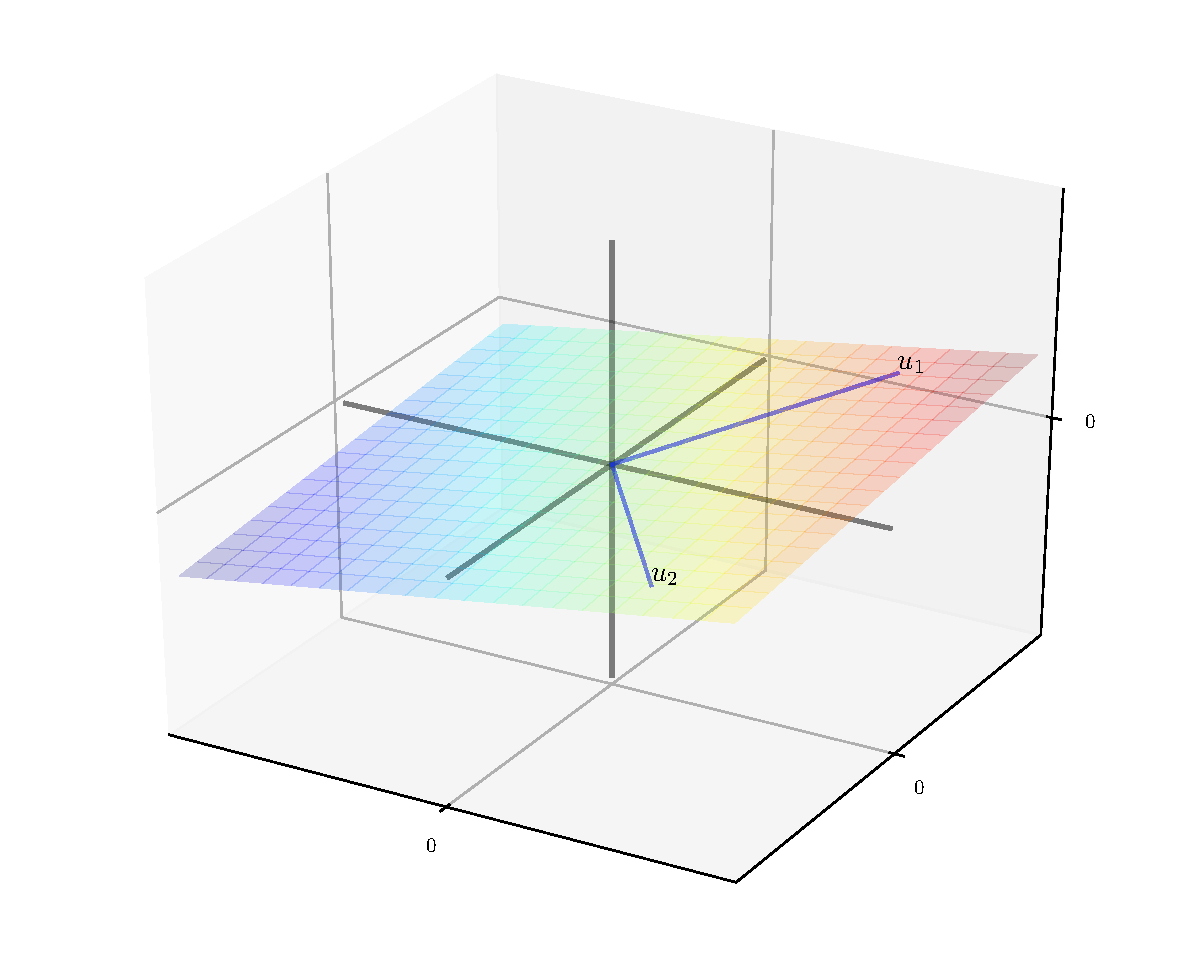
\includegraphics[width = 0.65\textwidth]{Ch4_files/Ch4_13_0.pdf}
    		\caption{Graphical Representation of the Span of $\mathbf{U}$}
    		\label{fig:span_graph}
    \end{figure}
    
    Let's take now however, the following set of vectors
\(\mathbf{U} = \{e_1, e_2, e_3\}\) (also called \emph{canonical basis})
where

\[
e_1 = \begin{pmatrix} 1 \\ 0 \\ 0 \end{pmatrix} \: , \: e_2 = \begin{pmatrix} 0 \\ 1 \\ 0 \end{pmatrix} \: , \: e_3 = \begin{pmatrix}  0 \\ 0 \\ 1 \end{pmatrix}
\]

The span of \(\mathbf{U}\) is now all \(\mathbb{R}^3\). Why? Note that
any \(x = (x_1, x_2, x_3)\in\mathbb{R}^3\) can be written as

\[
x = x_1 e_1 + x_2 e_2 + x_3 e_3
\]

However, if we take now \(\mathbf{U}_0 = \{e_1, e_2, e_1 + e_2\}\), if
\(y = (y_1, y_2, y_3)\) is any linear combination of these vectors,
then, it must be \(y_3 = 0\). Thus, the span of \(\mathbf{U}_0\) is no
longer \(\mathbb{R}^3\) but \(\mathbb{R}^2\). Why? Because the span will
be the set of all three-dimensional vectors whose third coordinate is
\(0\). However, for the first two coordinates, any vector can be
computed as a linear combination of them both.

To see this more clearly, note that what we are asked is to write any
vector \(y = (y_1, y_2, y_3)\) as a combination of the vectors
\(\mathbf{U}_0 = \{e_1, e_2, e_1 + e_2\}\), that is

\[
(y_1, y_2, y_3) = \beta_1 \begin{pmatrix} 1 \\ 0 \\ 0 \end{pmatrix} + \beta_2 \begin{pmatrix} 0 \\ 1 \\ 0 \end{pmatrix} + \beta_3 \begin{pmatrix} 1 \\ 1 \\ 0 \end{pmatrix}
\]

This can be written as the following system of equations

\begin{align*}
\beta_1 + \beta_3 &= y_1 \\
\beta_2 + \beta_3 &= y_2 \\
0 &= y_3
\end{align*}

Thus, this imposes that \(y_3 = 0\) if we want to create linear
combinations from this vector space. Furthermore, whatever values
\(\{y_1, y_2\}\) take, we can find \(\beta_1, \beta_2, \beta_3\) that
satisfy these equations.
\end{example}

\begin{definition}
A collection of vectors \(\mathbf{U} = \{\vec{\mathbf{u}}^1, \ldots, \vec{\mathbf{u}}^k\}\in\mathbb{R}^n\)
is said to be: 

\begin{itemize}
    \item\textbf{\emph{linearly dependent}} if some \emph{strict subset} of \(A\) has the same span as \(A\). 

    \item\textbf{\emph{linearly independent}} if it is not linearly dependent.
\end{itemize}
\end{definition}

This tells us that a set of vectors will be linearly independent if no
vector is \emph{redundant} to the span, linearly dependent otherwise.
This is easier to see if we take a look at the figure for the span of
vectors \(\{\vec{\mathbf{u}}^1, \vec{\mathbf{u}}^2\}\in\mathbb{R}^3\) as
a plane through the origin. Suppose we add a third vector to form the
set \(\{\vec{\mathbf{u}}^1, \vec{\mathbf{u}}^2, \vec{\mathbf{u}}^3\}\),
this set will be 

\begin{itemize}
    \item linearly dependent if \(\vec{\mathbf{u}}^3\) lies in the plane, because we could form it by using linear combinations of the other two vectors. 

    \item linearly independent otherwise.
\end{itemize}

\begin{theorem}
\(n\) vectors of \(n\) coordinates are linearly
dependent if and only if the determinant of the matrix they form is
zero.
\end{theorem}

\subsubsection{Rank}\label{rank}

\begin{definition}
Given a set of vectors \(\{\vec{\mathbf{u}}^1,\vec{\mathbf{u}}^2,\ldots,\vec{\mathbf{u}}^n\}\), the \textbf{rank} of this set is the maximum number of vectors that are
linearly independent among them.
\end{definition}

Thus, the rank of a matrix \(A\) is simply the \emph{dimension of its span}.

\begin{theorem}
Given a set of vectors \(\{\vec{\mathbf{u}}^1,\vec{\mathbf{u}}^2,\ldots,\vec{\mathbf{u}}^n\}\), and let \(A\) be the matrix formed with the columns of these vectors. Then, the rank of the vectors coincides with the order of the largest square submatrix of \(A\) with a determinant different from \(0\). 
\end{theorem}

Note that, from the discussion above, since \(\mathbb{R}^n\) can be
spanned by \(n\) vectors (take the example of the canonical basis), any
set of \(m > n\) vectors in \(\mathbb{R}^n\) must be linearly dependent.

\subsubsection{Rank of a matrix}\label{rank-of-a-matrix}

\begin{theorem}
Given an \(m\times n\) matrix \(A\), the rank of its \(m\) row vectors coincides with the rank of its \(n\) column vectors. This number is called \textbf{rank of matrix} \(A\) and it is denoted by \(\text{rk}(A)\).
\end{theorem}

\begin{example}
Compute the rank of the following matrix \[
A = \begin{pmatrix} 0 & 1 & -1 & 0 & 1 \\ 2 & 1 & 1 & -1 & 0 \\ 2 & 1 & 1 & 1 & 1 \end{pmatrix}
\]

Since the rank is the number of the linearly independent vectors in the
matrix, using the determinant of submatrices is useful to compute it.
Furthermore, there are more columns than rows, and there are \(3\) rows,
so the maximum possible rank is \(3\) (since the other vectors will be
linear combinations of the other three).

\begin{enumerate}
\def\labelenumi{\arabic{enumi}.}
\item
  The matrix has non-zero elements, thus, \(\text{rk}(A) \geq 1\). Let
  us start by choosing as non-zero element \(a_{12}\).
\item
  Choose a \(2\times 2\) submatrix, i.e.,
  \(B = \begin{pmatrix} a_{11} & a_{12} \\ a_{21} & a_{22} \end{pmatrix} = \begin{pmatrix} 0 & 1 \\ 2 & 1 \end{pmatrix}\).
  Since \(\det(B) = -2\), \(\text{rk}(A) \geq 2\).
\item
  Note that computing the determinant of
  \(C = \begin{pmatrix} a_{11} & a_{12} & a_{13}\\ a_{21} & a_{22} & a_{23} \\ a_{31} & a_{32} & a_{33}\end{pmatrix}\)
  would give us \(0\). Does that mean that the rank is \(2\)? Not
  necessarily, since we should test for \textbf{all possible}
  submatrices. However, we can take instead, the submatrix
  \(D = \begin{pmatrix} a_{11} & a_{12} & a_{15}\\ a_{21} & a_{22} & a_{25} \\ a_{31} & a_{32} & a_{35}\end{pmatrix}\)
  which contains previous submatrices. Note further that
  \(\det(D) = -2\) which implies that the rank of the matrix is
  \(\text{rk} = 3\) since it cannot be greater than that.
\end{enumerate}
\end{example}

\begin{definition}
A square matrix whose rank equals the number of its rows (or columns) is said to be a \textbf{nonsingular matrix}. Thus, if the determinant of the matrix is not zero, then the matrix is nonsingular, otherwise, it is said to be \emph{singular}.
\end{definition}

\subsection{Systems of Equations}\label{systems-of-equations}

\subsubsection{Matrices as maps}\label{matrices-as-maps}

Each \(n\times k\) matrix \(A\) can be identified with a function
\(f(x) = Ax\) mapping \(x\in\mathbb{R}^k\) into
\(y = Ax \in\mathbb{R}^n\). The property that characterizes these
functions is that they are \textbf{\emph{linear}}.

\begin{definition}
\textbf{Definition:} A function
\(f : \mathbb{R}^k \rightarrow \mathbb{R}^n\) is called
\textbf{\emph{linear}} if \(\forall \: x,y\in\mathbb{R}^k\) and
\(\alpha,\beta\in\mathbb{R}\) we have

\[
f(\alpha x + \beta y) = \alpha f(x) + \beta f(y)
\]
\end{definition}

This holds for the function \(f(x) = Ax + b\) when \(b\) is the zero
vector, and fails when \(b\) is non-zero. Actually, \(f\) will be linear
if and only if there exists a matrix \(A\) such that
\(f(x) = Ax \: \forall x\).

\subsubsection{Systems of Equations}\label{systems-of-equations-1}

We introduced systems of equations in the Introduction and we also
introduced the idea that linear systems can be represented by matrices.
It should be apparent now that we know matrix operations why the system
of the introduction could be written as

\[
\begin{pmatrix} x_{t+1} \\ y_{t+1} \end{pmatrix} = \begin{pmatrix} q & p \\ 1-q & 1-p \end{pmatrix}\begin{pmatrix} x_t \\ y_t \end{pmatrix}
\]

Generally, we can write any linear system as

\[
y = Ax
\]

Where \(y\) is an \(n\times 1\) vector, \(A\) is an \(n\times k\)
matrix, and \(x\) is a \(k\times 1\) vector. The problem is to find a
vector \(x\in\mathbb{R}^k\) that solves the equation taking \(A\) and
\(y\) as given. What are the conditions on \(A\) such that a solution
exists and it is unique?

First of all, we should note that \(Ax\) is a linear combination of the
columns of \(A\), hence, the range of the function \(f(x) = Ax\) is
precisely the span of the columns of \(A\). The larger the span of \(A\)
the more likely it will be that it contains an arbitrary \(y\).
Therefore, the ideal is that the columns of \(A\) are \textbf{linearly
independent}. In fact, if the column vectors forming \(A\) are linearly
independent and \(y = Ax = x_1 a_1 + \ldots + x_k a_k\), then there is
no \(z\neq x\) such that \(y = Az\), therefore, linearly independent
column vectors will give us a unique solution.

A system of linear equations written in matrix form can also be
represented by an \textbf{augmented} matrix with the vector of
independent terms \((y)\) included as a column in matrix \(A\), i.e.,

\[
[A,y] = \left(\begin{array}{cccc|c}
a_{11} & a_{12} & \ldots & a_{1k} & y_1 \\ 
a_{21} & a_{22} & \ldots & a_{2k} & y_2 \\ 
\vdots & \vdots & \ddots & \vdots & \vdots \\ 
a_{n1} & a_{n2} & \ldots & a_{nk} & y_n 
\end{array}
\right)
\]

\begin{definition}
A system of equations \(y = Ax\) is said to be
\textbf{homogeneous} if all the vector of independent terms is the zero
vector, i.e., \(y = \mathbf{0}\).
\end{definition}

\begin{definition}
A system of equations \(y = Ax\) is said to be
\textbf{incompatible} if it has no solution. If any solution exists,
then it is called \textbf{compatible}. Depending on the number of
solutions, a system can be: 
\begin{itemize}
    \item \textbf{Determinate compatible} if it only has one solution. 
    \item \textbf{Indeterminate compatible} if it has infinite solutions.
\end{itemize}
\end{definition}

\paragraph{\texorpdfstring{The \(n\times n\)
Case}{The n\textbackslash{}times n Case}}\label{the-ntimes-n-case}

Let us have an \(n\times n\) matrix \(A\), then if the columns of \(A\)
are linearly independent then, their span is \(\mathbb{R}^n\), and thus,
the range of \(f(x) = Ax\) is \(\mathbb{R}^n\) as well. Therefore, we
can always find an \(x\) such that the equation \(y = Ax\) is satisfied.
Furthermore, this solution is \textbf{unique}. The property of having
linearly independent columns is called \textbf{\emph{having full column
rank}}.

However, even if we know the solution exists and it is unique, how do we
compute it? Suppose that \(y\) and \(A\) are scalars, then the equation
\(y = Ax\) is solved by \(x = A^{-1}y\) as long as \(A\neq 0\). For
matrices, a similar solution exists if the \textbf{inverse} of \(A\)
exists. Then, if the inverse of \(A\) exists, the solution to the system
is given by

\[
x = A^{-1}y
\]

Note that the multiplication order \textbf{matters} for this operation.

    \paragraph{More rows than columns}\label{more-rows-than-columns}

Suppose we have now an \(n\times k\) matrix \(A\) for which \(n > k\),
this is the typical case of linear regression when the number of
observations is larger than the number of explanatory variables). Given
a particular vector \(y\in\mathbb{R}^n\) we are looking for a certain
\(x\in\mathbb{R}^k\) such that the equation \(y = Ax\) is satisfied. The
existence of a solution is highly unlikely in this case, however, let us
further assume that the columns of \(A\) are linearly independent, thus,
the span of \(A\) is a \(k-\)dimensional subspace of \(\mathbb{R}^n\).
Therefore, it will be very unlikely if any arbitrary
\(y\in\mathbb{R}^n\) is contained in that subspace. It is useful again
to revisit previous figure and think how likely it would be for an
arbitrary vector \(y\in\mathbb{R}^3\) to lie exactly somewhere in the
span of \(\{\vec{\mathbf{u}}^1,\vec{\mathbf{u}}^2\}\), furthermore
taking into account that this plane has zero \emph{"thickness"}.

Since, in linear regression, this is the usual context the approach is
to find a \emph{"best approximation"} to the solution, typically making
the distance \(||y - Ax||\) as small as possible. You will see more on
this topic further on.

\paragraph{More columns than rows}\label{more-columns-than-rows}

Take now an \(n\times k\) matrix \(A\) for which \(n < k\). In this
case, we have less equations than unknowns. In this case, we will have
either no solutions or infinitely many. Take for example a matrix
\(2\times 3\), thus the set can never be linearly independent since the
matrix is composed by 3 vectors in \(\mathbb{R}^2\) which implies that
it is always possible to find two vectors that span \(\mathbb{R}^2\).

\subsubsection{Rouché-Frobenius
Theorem}\label{rouchuxe9-frobenius-theorem}

It is important to rationalize all these ideas in one single theorem to
analyse systems of equations.

\begin{theorem}
Given a system of equations \(Ax = y\) with \(n\)
equations and \(k\) unknowns, i.e. \(A\) is of order \(n\times k\),
\(y\) is an \(n\times 1\) vector, and \(x\) is a \(k\times 1\) vector,
then:

\begin{enumerate}
\def\labelenumi{\arabic{enumi}.}
\item
  If \(\text{rk}(A) \neq \text{rk}\left([A,y]\right)\) the system is
  \textbf{incompatible}.
\item
  If \(\text{rk}(A) = \text{rk}\left([A,y]\right)\) the system is
  \textbf{compatible}.
\item
  If \(\text{rk}(A) = \text{rk}\left([A,y]\right) = n\) the system is
  \textbf{determinate compatible}.
\item
  If \(\text{rk}(A) = \text{rk}\left([A,y]\right) < n\) the system is
  \textbf{indeterminate compatible}.
\end{enumerate}
\end{theorem}

Let's build up on intuition, if we have a system \(Ax = y\), the rank of
matrix \(A\) will always be smaller or equal to the rank of the
augmented matrix since the latter has \textbf{all columns} of \(A\) and
an additional one, and recall that the rank of a matrix is just the
\textbf{dimension of its span}. If the system does have a solution, it
means that vector \(y\) is \textbf{linearly dependent} on the columns of
matrix \(A\) which would tell us that the rank of the augmented matrix
is the same as the rank of matrix \(A\). If the system does not have a
solution, it means that the rank of the augmented matrix will be larger
than that of matrix \(A\) which implies that vector \(y\) is \textbf{not
linearly dependent} on the columns of \(A\).

Conditioning on having at least one solution, i.e. both ranks are equal,
the possibility of having a unique solution arises when there are the
same number of rows and columns because the columns of \(A\) span all
\(\mathbb{R}^n\) so it is always possible to find a solution satisfying
the equation.

\textbf{Note:} The solution of systems of equations is indeed a very
important and interesting subject, however, it is a topic that should be
familiar to all of you by now. The two basic procedures through which
systems are typically analysed are \emph{Gauss and Gauss-Jordan
Elimination} and \emph{Cramer systems}. The first one is based on
transforming the matrix into a simpler one, typically a lower triangular
matrix or transform it into a \emph{row echelon form}. Cramer systems
are based on properties of the determinants of the so called
\emph{Cramer's rule} which is based on the computation of determinants
by substituting vector \(y\) column by column. You can read on this in
any textbook, for Gauss-Jordan elimination, I like the exposition in
Simon, C. P., \& Blume, L. (1994). Mathematics for economists (Ch. 7).
The same reference also explains Cramer's rule in Ch.9.


\section{Eigenvalues and
Eigenvectors}\label{eigenvalues-and-eigenvectors}

In economic theory, constantly appear dynamic models (think of the Solow
growth model, for example). In the context of linear dynamic models, the
eigenvalues are the components of the explicit solutions, while in
nonlinear dynamic models, the signs of the eigenvalues determine the
stability of equilibria. Over the year you will see more on this.

Essentially, the eigenvalues of a given \(n\times n\) matrix are the
\(n\) numbers that summarize the most important properties of that
matrix that is why they are also called \emph{characteristic values}. In
this section, we will mostly learn what these eigenvalues really are,
how to compute them, and some properties of these objects.

\subsection{Definition and Intuition}\label{definition-and-intuition}

\begin{definition}
Let \(A\) be a square matrix. An \textbf{eigenvalue} of \(A\) is a number \(\lambda\) which, when subtracted from each of the diagonal entries of \(A\), converts \(A\)
into a singular matrix. Thus, \(\lambda\) is an eigenvalue of \(A\) if
and only if \(A-\lambda I\) is a singular matrix.
\end{definition}

\begin{example}
Let's look for the eigenvalues of the \emph{diagonal matrix} \(\begin{pmatrix} 2 & 0 \\ 0 & 3 \end{pmatrix}\).

\begin{itemize}
\item
  Subtracting \(2\) from the main diagonal yields
  \(\begin{pmatrix} 0 & 0 \\ 0 & 1 \end{pmatrix}\).
\item
  Subtracting \(3\) from the main diagonal yields
  \(\begin{pmatrix} -1 & 0 \\ 0 & 0 \end{pmatrix}\).
\end{itemize}

Thus, \(2\) and \(3\) are eigenvalues of
\(\begin{pmatrix} 2 & 0 \\ 0 & 3 \end{pmatrix}\). In fact, this is a
general property of diagonal matrices.
\end{example}

\begin{theorem}
The diagonal entries of a diagonal matrix \(\mathcal{D}\) are eigenvalues of \(\mathcal{D}\).
\end{theorem}

\begin{theorem}
A square matrix \(A\) is singular if and only if \(0\) is an eigenvalue of \(A\).
\end{theorem}

\begin{proof}
These two theorems are straightforward consequences of the definition of
eigenvalue.
\end{proof}

\subsection{Finding the Eigenvalues}\label{finding-the-eigenvalues}

Since it is difficult to try matrices to find the eigenvalues, it is
useful to find a systematic way of finding them. The key of the
definition of the eigenvalue is that the matrix resulting from
subtracting to the elements of the main diagonal a particular value is
\emph{singular}. A matrix is singular if and only if its determinant is
\(0\). Therefore, \(\lambda\) is an eigenvalue of \(A\) if and only if

\[
det(A-\lambda I) = 0
\]

For an \(n\times n\) matrix \(A\), the left-hand side of the equation is
a polynomial of \(n-\)th degree in the variable \(\lambda\) (which is
what we are looking for). This polynomial is called
\textbf{characteristic polynomial} of \(A\). Then, \(\lambda\) will be
an eigenvalue if and only if it is a root of the characteristic
polynomial of \(A\).

\begin{example}
Take a \(2\times 2\) matrix, its characteristic
polynomial will be

\[
det(A-\lambda I)  = det\begin{pmatrix} a_{11}-\lambda & a_{12} \\ a_{21} & a_{22}-\lambda \end{pmatrix} = \lambda^2 - (a_{11}+a_{22})\lambda + (a_{11}a_{22}-a_{12}a_{21})
\]

Which is a second order polynomial.
\end{example}

Note that an \(n-\)th order polynomial has at most \(n\) roots (exactly
\(n\) if one counts roots with their multiplicity and counts complex
roots). Thus, an \(n\times n\) matrix has at most \(n\) eigenvalues.

\begin{theorem}
A square matrix \(B\) is nonsingular if and only if the
only solution of \(B\mathbf{x} = \mathbf{0}\) is
\(\mathbf{x} = \mathbf{0}\).
\end{theorem}

\begin{proof}

\begin{enumerate}
\def\labelenumi{\arabic{enumi}.}
\item
  \(B\) is nonsingular \(\rightarrow\) only solution is
  \(\mathbf{x} = 0\).

  \begin{align*}
  B\mathbf{x} &= \mathbf{0} \\
  B^{-1}B\mathbf{x} &= \mathbf{0} \\
  \mathbf{x} &= \mathbf{0}
  \end{align*}
\item
  The only solution is \(\mathbf{x} = 0 \rightarrow\) \(B\) is
  nonsingular.

  If \(\mathbf{x}\) is not the trivial solution, then the columns of \(B\) are linearly dependent (recall the definition of a set of vectors that are linearly dependent). Then, \(\det(B) = 0\Rightarrow B\) is singular. Thus, if the only solution is \(\mathbf{x} = \mathbf{0}\), then \(B\) is
nonsingular.
\end{enumerate}
\end{proof}

The fact that \(A-\lambda I\) is singular when \(\lambda\) is an
eigenvalue of \(A\) means that the system of equations
\((A-\lambda I)\mathbf{v} = \mathbf{0}\) has a solution different than
\(\mathbf{v} = \mathbf{0}\). Therefore, we have the following definition.

\begin{definition}
When \(\lambda\) is an eigenvalue of \(A\), a \emph{nonzero} vector \(\mathbf{v}\) such that

\[
(A-\lambda I)\mathbf{v} = \mathbf{0}
\]

is called \textbf{eigenvector} of \(A\) corresponding to eigenvalue
\(\lambda\). In turn, this implies that

\[
A\mathbf{v} = \lambda \mathbf{v}
\]
\end{definition}

What this in turn tells us is that an eigenvector of \(A\) is a vector
such that when the map \(f(\mathbf{x}) = A\mathbf{x}\) is applied,
\(\mathbf{v}\) is simply scaled. The next figure shows two eigenvectors
(in blue) and their images under \(A\) (in red).

    \begin{figure}[htbp]
    	\centering 
    		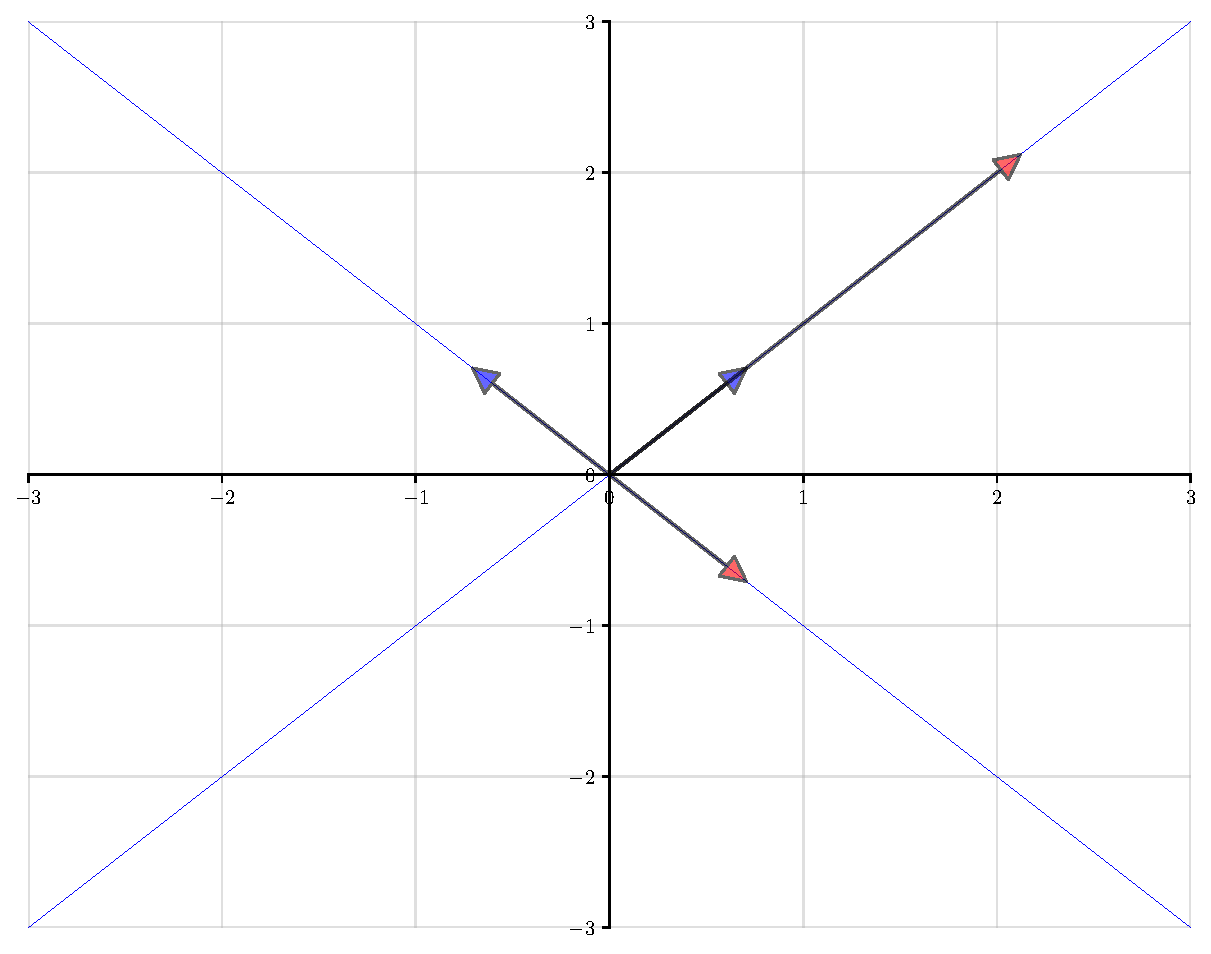
\includegraphics[width = 0.65\textwidth]{Ch4_files/Ch4_18_0.pdf}
    		\caption{Eigenvectors and their Images under $A$}
    		\label{fig:eigenvectors}
    \end{figure}
    
\subsection{Diagonalization}\label{diagonalization}

Note that from the equation \(A\mathbf{v} = \mathbf{v}\lambda\) every
\(\lambda\) determines an \(n\times 1\) column vector (since \(A\) is
\(n\times n\), \(\mathbf{v}\) is \(n\times 1\), and \(\lambda\) is a
scalar). Therefore, we can rewrite the equation in matrix form as

\[
AV = VD
\]

Where \(V\) is the \(n\times n\) matrix formed by the eigenvectors of
\(A\), and \(D\) is an \(n\times n\) diagonal matrix with the
eigenvalues of \(A\) in the main diagonal. If the eigenvectors of \(A\)
are linearly independent then, \(\det(V) \neq 0\), and \(V\) can be
inverted yielding:

\[
V^{-1}AV = D
\]

Which tells us that if we pre-multiply \(A\) with the inverse
of \(V\) and post-multiply with $V$, we get a diagonal matrix with its eigenvalues as diagonal
elements. This is called \textbf{\emph{diagonalization}} of matrix
\(A\).

\begin{theorem}
Let \(A\) be an \(n\times n\) matrix. If \(A\) has
\(n\) distinct eigenvalues \(A\) is diagonalizable.
\end{theorem}

\begin{example}
Take a matrix \(A = \begin{pmatrix} 0.06 & -1 \\ -0.004 & 0 \end{pmatrix}\). Let's
compute the eigenvalues, eigenvectors, and the diagonal matrix
associated to \(A\).

\begin{itemize}
\item
  Let us start by declaring the system of equations
\end{itemize}

\[
(A - \lambda I) \mathbf{v} = \begin{pmatrix} 0.06 - \lambda & -1 \\ -0.004 & 0 - \lambda \end{pmatrix} \begin{pmatrix} v_1 \\ v_2 \end{pmatrix} = 0
\]

\begin{itemize}
\item
  We need to get a \textbf{\emph{non trivial solution}} in which
  \(\mathbf{v}\neq 0\). To get that, we need that
  \(\det(A-\lambda I) = 0\).
\end{itemize}

\[
\lambda^2 - 0.06\lambda -0.004 = 0
\]

    Which is satisfied for \(\lambda_1 = 0.1\) and \(\lambda_2 = -0.04\).
The diagonal matrix associated to \(A\) is thus

\[
D = \begin{pmatrix} 0.1 & 0 \\ 0 & -0.04 \end{pmatrix}
\]

To find the eigenvector associated with the eigenvalue
\(\lambda_1 = 0.1\), substitute it in matrix \(A-\lambda_1 I\) and
compute

\[
\begin{pmatrix} 0.06-0.1 & -1 \\ -0.004 & 0 - 0.1 \end{pmatrix}\begin{pmatrix} v_{11} \\ v_{21} \end{pmatrix} = 0
\]

This is a system of equations with two unknowns and the equations are

\begin{align*}
-0.04 v_{11} - v_{21} &= 0 \\
-0.004 v_{11} - 0.1 v_{21} &= 0 
\end{align*}

Note that the second equation is a linear combination of the first one,
thus can be ignored. The solution for \(v_{11}\) and \(v_{21}\) will be
unique only up to an arbitrary scalar multiple of each value. We can
\emph{normalize} \(v_{11} = 1\) and thus obtain \(v_{21} = -0.04\), and
we get the first eigenvector.

Repeating the process for \(\lambda_2 = -0.04\), yields the system

\begin{align*}
0.1 v_{12} - v_{22} &= 0 \\
-0.004 v_{12} + 0.04 v_{22} &= 0
\end{align*}

Note again that the second equation is \((-0.04)\times\) first equation.
Again, normalizing \(v_{12} = 1\) yields \(v_{22} = 0.1\). Therefore,
the matrix of normalized eigenvectors is given by

\[
V = \begin{pmatrix} 1 & 1 \\ -0.04 & 0.1 \end{pmatrix}
\]

It is easy to verify that now \(V^{-1}AV = D\).
\end{example}

\section{Quadratic Forms}\label{quadratic-forms}

The original purpose of economics is the study of how economic agents
behave in economically relevant areas. For example, in microeconomics we
focus on the analysis of individuals and markets, while macroeconomics
analyses the aggregate economy, a set of individuals. To do so, one of
the cornerstone ideas is that of \textbf{optimization}, which is
basically try to maximize or minimize some outcome with certain
restrictions. The simplest form of optimization problems is the
optimization of \emph{quadratic forms}. They are the simplest and they
have matrix representations.

\subsection{Introduction and
Definition}\label{introduction-and-definition}

A quadratic function in one variable can be described by
\(f(x) = ax^2\), while the natural generalization of a quadratic to two
variables is the quadratic form

\[
Q(x_1, x_2) = a_{11}x_1^2 + a_{12}x_1 x_2 + a_{22} x_2^2
\]

Note that the sum of exponents in each of the terms is two. In three
variables, we could generalize it to be

\[
Q(x_1, x_2, x_3) = a_{11}x_1^2 + a_{12}x_1 x_2 + a_{13}x_1 x_3 + a_{22} x_2^2 + a_{23}x_2 x_3 + a_{33} x_3^2
\]

To generalize for \(k\) variables, we have the following definition.

\begin{definition}
A \textbf{quadratic form} on \(\mathbb{R}^k\) is a
real-valued function of the form

\[
Q(x_1, \ldots, x_k) = \sum^k_{i,j = 1} a_{ij}x_i x_j
\]
\end{definition}

\subsection{Matrix representation}\label{matrix-representation}

Let us start by taking again a linear function on \(k\) variables i.e.,
\(f(x) = a_1 x_1 + \cdots + a_k x_k\).

\begin{theorem}
Let \(f \: : \: \mathbb{R}^k \rightarrow \mathbb{R}\) be a linear function. Then, there exists a vector \(\mathbf{a}\in\mathbb{R}^k\) such that \(f(\mathbf{x}) = \mathbf{a}\cdot\mathbf{x}\) for all \(\mathbf{x}\in\mathbb{R}^k\).
\end{theorem}

\begin{proof}
For simplicity, let \(k = 3\) and recall the discussion
on the canonical basis. Then,

\[
\mathbf{x} = x_1\begin{pmatrix} 1 \\ 0 \\ 0 \end{pmatrix} + x_2 \begin{pmatrix} 0 \\ 1 \\ 0 \end{pmatrix} + x_3 \begin{pmatrix} 0 \\ 0 \\ 1 \end{pmatrix}
\]

Since \(f(\cdot)\) is linear, and let

\[
\mathbf{e}_1 = \begin{pmatrix} 1 \\ 0 \\ 0 \end{pmatrix} \qquad \mathbf{e}_2 \begin{pmatrix} 0 \\ 1 \\ 0 \end{pmatrix} \qquad \mathbf{e}_3 \begin{pmatrix} 0 \\ 0 \\ 1 \end{pmatrix}
\]

then

\begin{align*}
f(\mathbf{x}) &= x_1 f(\mathbf{e}_1) + x_2 f(\mathbf{e}_2) + x_3 f(\mathbf{e}_3) \\
& = x_1 a_1 + x_2 a_2 + x_3 a_3 \\
& = \mathbf{a}\cdot\mathbf{x} \\
& = \begin{pmatrix} a_1 & \cdots & a_k \end{pmatrix} \begin{pmatrix} x_1 \\ \vdots \\ x_k \end{pmatrix}
\end{align*}
\end{proof}

Just as this representation holds for linear functions, quadratic forms
also have matrix representations. Before going to the general theorem
discussing the matrix representation of quadratic forms, let's think of
the quadratic form in \(\mathbb{R}^2\).

\[
Q(x_1, x_2) = a_{11}x_1^2 + a_{12}x_1 x_2 + a_{22} x_2^2 = \begin{pmatrix} x_1 & x_2 \end{pmatrix} \begin{pmatrix} a_{11} & a_{12} \\ 0 & a_{22}\end{pmatrix} \begin{pmatrix} x_1 \\ x_2 \end{pmatrix}
\]

Note that an equivalent representation of that quadratic form is

\[
Q(x_1, x_2) = \begin{pmatrix} x_1 & x_2 \end{pmatrix} \begin{pmatrix} a_{11} & \dfrac{1}{2}a_{12} \\ \dfrac{1}{2}a_{12} & a_{22}\end{pmatrix} \begin{pmatrix} x_1 \\ x_2 \end{pmatrix}
\]

Analogously, in \(\mathbb{R}^3\)

\[
Q(x_1, x_2) = \begin{pmatrix} x_1 & x_2 & x_3\end{pmatrix} \begin{pmatrix} a_{11} & \dfrac{1}{2}a_{12} & \frac{1}{2} a_{13} \\ \frac{1}{2}a_{12} & a_{22} & \frac{1}{2}a_{23} \\ \frac{1}{2}a_{13} & \frac{1}{2} a_{23} & a_{33}\end{pmatrix} \begin{pmatrix} x_1 \\ x_2 \\ x_3 \end{pmatrix}
\]

Through this procedure, we can prove the following theorem about
quadratic forms as matrix forms.

\begin{theorem}
The general quadratic form

\[
Q(x_1, \ldots, x_n) = \sum_{i\leq j} a_{ij}x_i x_j
\]

Can be written as

\[
Q(x_1, \ldots, x_n) = \begin{pmatrix} x_1 & x_2 & \cdots & x_n \end{pmatrix} \begin{pmatrix} a_{11} & \dfrac{1}{2}a_{12} & \cdots & \dfrac{1}{2} a_{1n} \\ \dfrac{1}{2}a_{12} & a_{22} & \cdots & \dfrac{1}{2}a_{2n}\\ \vdots & \vdots & \ddots & \vdots \\ \dfrac{1}{2}a_{1n} & \dfrac{1}{2} a_{2n} & \cdots & a_{nn}\end{pmatrix} \begin{pmatrix} x_1 \\ x_2 \\ \cdots \\ x_n \end{pmatrix}
\]

Which is equivalent to

\[
Q(\mathbf{x}) = \mathbf{x}'A\mathbf{x}
\]

Where \(A\) is a unique symmetric matrix. Conversely, if \(A\) is a
symmetric matirx, then the real-valued function
\(Q(\mathbf{x}) = \mathbf{x}'A\mathbf{x}\) is a quadratic form.
\end{theorem}

\subsection{Definiteness of Quadratic
Forms}\label{definiteness-of-quadratic-forms}

Note that a particular property of quadratic forms is that when
\(\mathbf{x} = \mathbf{0}\) the quadratic form also takes value zero. In
one variable, the quadratic form \(f(x) = ax^2\) takes always
non-negative values if \(a > 0\). Such a form is called \textbf{positive
definite}; and zero is its \textbf{\emph{global minimizer}}. Conversely,
if \(a < 0\) the function always takes non-positive values, thus it
takes the name \textbf{negative definite}; and zero is its
\textbf{\emph{global maximizer}}.

Similarly, in two dimensions, the quadratic form
\(Q(x_1, x_2) = x_1^2 + x_2^2\) is always greater than zero at any
\((x_1, x_2) \neq (0, 0)\), thus it is also called \textbf{positive
definite}. The quadratic form \(Q(x_1, x_2) = - x_1^2 - x_2^2\) is
called \textbf{negative definite}. Those forms that take on negative and
positive values are called \textbf{indefinite}, an example
\(Q(x_1, x_2) = x_1^2 - x_2^2\).

There are although two intermediate cases:

\begin{enumerate}
\def\labelenumi{\arabic{enumi}.}
\item
  A quadratic form which is always \(\geq 0\) but might be equal to zero
  at some \(\mathbf{x} \neq \mathbf{0}\). In this case, we call them
  \textbf{positive semidefinite}. An example is \[
  Q(x_1, x_2) = (x_1 + x_2)^2 = x_1^2 + 2x_1x_2 + x_2^2
  \] Note that at \((1, -1)\) or \((-2, 2)\) the quadratic function
  takes value zero.
\item
  A quadratic form which is always \(\leq 0\) but might be equal to zero
  at some \(\mathbf{x} \neq \mathbf{0}\). In this case, we call them
  \textbf{negative semidefinite}. An example is \[
  Q(x_1, x_2) = -(x_1 + x_2)^2
  \]
\end{enumerate}

The following figure represents these cases.

    \begin{figure}[htbp]
    	\centering 
    		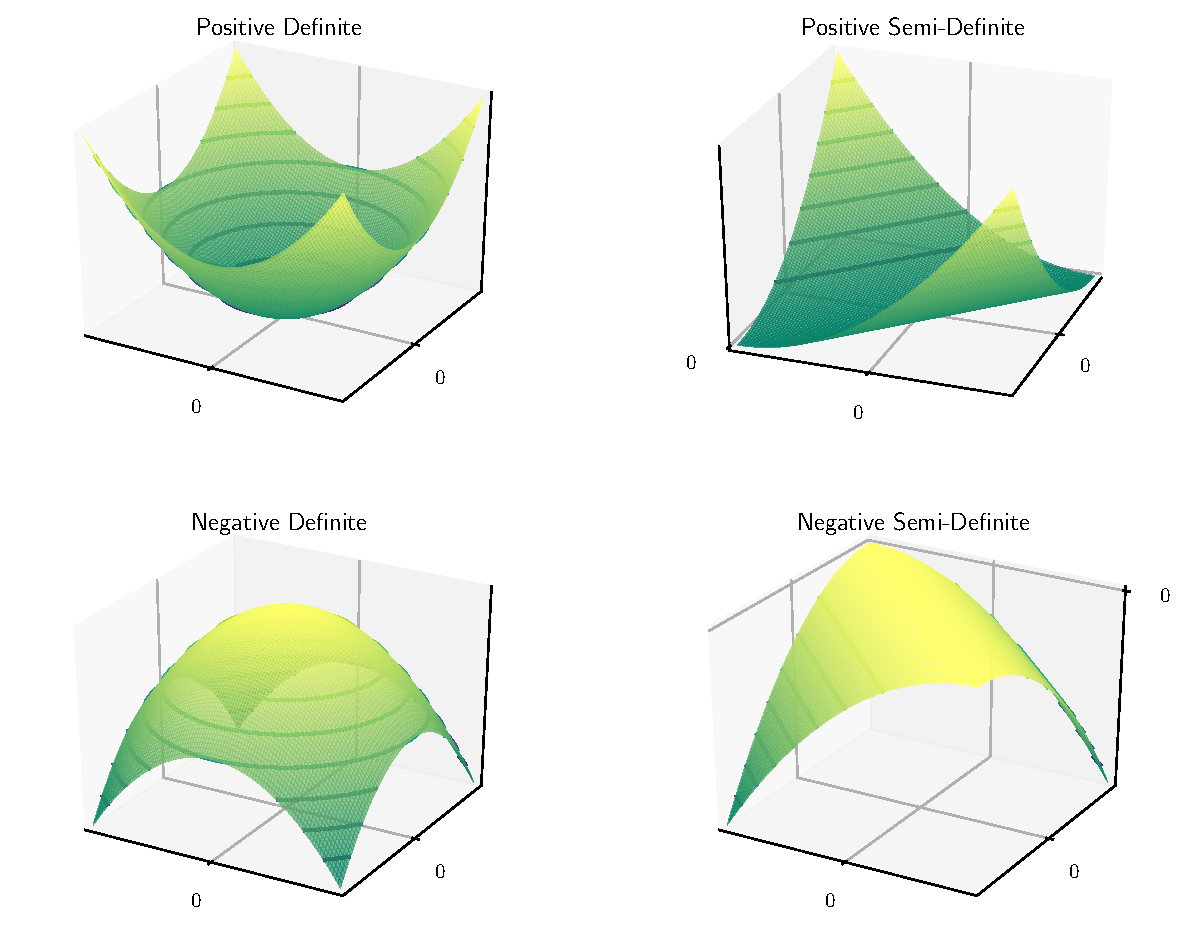
\includegraphics[width = 0.65\textwidth]{Ch4_files/Ch4_21_0.pdf}
    		\caption{Graphs of Quadratic Froms}
    		\label{fig:quad_forms}
    \end{figure}
    
    \subsubsection{Definite Symmetric
Matrices}\label{definite-symmetric-matrices}

A symmetric matrix is called positive (negative) (semi)definite
according to the definiteness of the corresponding quadratic form
\(Q(\mathbf{x}) = \mathbf{x}'A\mathbf{x}\).

\begin{definition}
Let \(A\) be an \(n\times n\) symmetric matrix,
then \(A\) is:

\begin{itemize}
\item
  \textbf{Positive definite} if
  \(\mathbf{x}'A\mathbf{x} > 0 \: \forall \: \mathbf{x} \neq \mathbf{0}\in\mathbb{R}^n\),
\item
  \textbf{Positive semidefinite} if
  \(\mathbf{x}'A\mathbf{x} \geq 0 \: \forall \: \mathbf{x} \neq \mathbf{0}\in\mathbb{R}^n\),
\item
  \textbf{Negative definite} if
  \(\mathbf{x}'A\mathbf{x} < 0 \: \forall \: \mathbf{x} \neq \mathbf{0}\in\mathbb{R}^n\),
\item
  \textbf{Negative semidefinite} if
  \(\mathbf{x}'A\mathbf{x} \leq 0 \: \forall \: \mathbf{x} \neq \mathbf{0}\in\mathbb{R}^n\),
\item
  \textbf{Indefinite} if \(\mathbf{x}'A\mathbf{x} > 0\) for some
  \(\mathbf{x} \neq \mathbf{0}\in\mathbb{R}^n\) and,
  \(\mathbf{x}'A\mathbf{x} < 0\) for other \(\mathbf{x}\in\mathbb{R}^n\)
\end{itemize}
\end{definition}

\textbf{Application:} The same as for one variable functions, the sign
of the second derivative of a function at a critical point gives a
necessary and a sufficient condition for determining whether that
critical point is a maximum, a minimum, or neither. The generalization
of this to a multivariate case, involves checking whether the Hessian
(matrix of second derivatives) is positive definite, negative definite,
or indefinite at a critical point. Furthermore, a function is concave in
a certain region if the Hessian is \emph{negative semidefinite} for all
\(\mathbf{x}\) in that region.

\end{document}